\documentclass{article}

\usepackage{apacite} % For the bibliography
\usepackage{graphicx} % For including graphics
\usepackage{lipsum} % To add some latin random text

\begin{document}

\section*{The beginning...} 


%%%% ADD SOME CITATIONS (THE FIRST = IN-TEXT. THE SECOND = INDIRECT)
\citeA{huntington1993clash} says a lot of things. Things are not always what we want them to be \cite{skocpol1999bringing}.

\citeA{kennedy2004decline} says that blablabla



%%%% ADD RANDOM LATIN TEXT
\lipsum[1]


%%%% ADD OUR TWO FIGURES
\begin{figure}[h!]
  \caption{My Super Histogram}
  \centering
  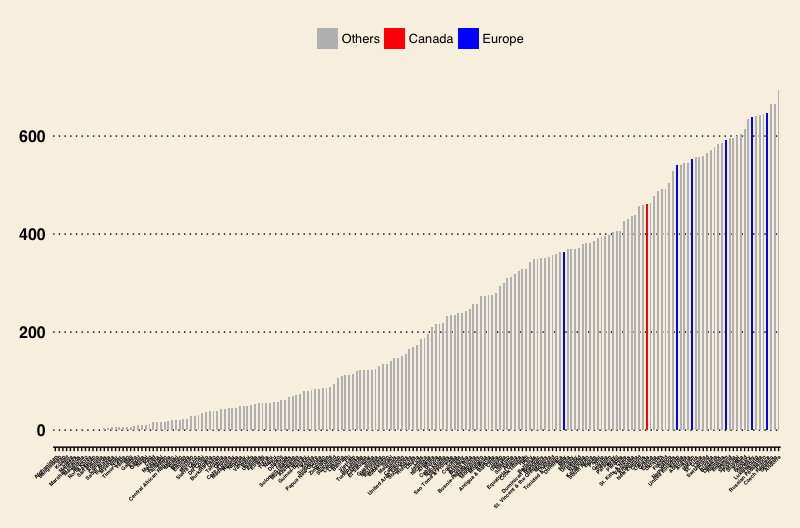
\includegraphics[width=1\textwidth]{AlcoholConsumptionHistogram}
\end{figure}

\begin{figure}[h!]
  \caption{My Super Map}
  \centering
  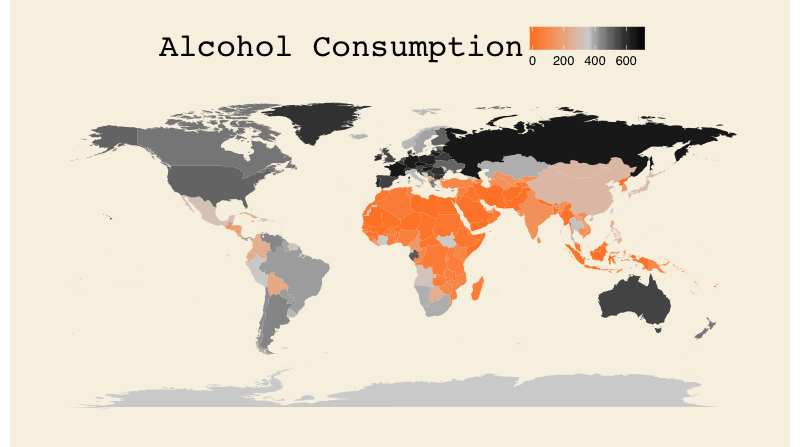
\includegraphics[width=1\textwidth]{AlcoholConsumptionMap}
\end{figure}


%%%% ADD RANDOM LATIN TEXT
\lipsum[2]


%%%% ADD A REGRESSION TABLE



%%%% PRINT THE BIBLIOGRAPHY
\bibliographystyle{apacite}
\bibliography{MyBibliography}

\end{document}




